\documentclass{article}
\usepackage[utf8]{inputenc}
\usepackage[T1]{fontenc}
\usepackage{amsmath}
\usepackage{parskip}
\usepackage{hyperref}
\usepackage{graphicx}
\usepackage{tikz}
\usetikzlibrary{calc,positioning}
\usepackage[ruled,vlined]{algorithm2e}

\def\layersep{2.5cm}

\SetKwProg{Fn}{Function}{ is}{}
\newcommand{\SetAlgoStyle}{
	\SetAlgoNoLine
	\SetAlgoNoEnd
	\DontPrintSemicolon
}

\newcommand{\fig}[2]{
	\begin{figure}[!htb]
		\center{\includegraphics[width=0.75\textwidth,keepaspectratio]{res/#1}}
		\caption{\label{fig:caption} #2}
	\end{figure}
}

\title{SGSN word embedder optimization}
\author{Lazar Jelić}
\date{\today}

\begin{document}

\maketitle

\begin{abstract}

This note provides new insight on time and memory optimization techniques for
skip-gram word embedding neural network with autoencoder architecture.

\end{abstract}

\section{Introduction}

There are some ways to optimize computations and memory usage in the
original word2vec implementation. In this note we explore some of them. Source
code can be found at \url{https://github.com/jelic98/raf_nlp}.

\section{Implementation}

We've implemented the following word embedder using C programming language.

\subsection{Network architecture}

As in the original word2vec implementation, we are using autoencoder
architecture which is capable of discovering structure within data in order
to develop a compressed representation of the input. If we pass word from
vocabulary to the input layer, then this representation will be word embedding.

\medbreak

Network consists of $3$ layers and $2$ weight matrices between them.

The first layer is the input layer which is onehot vector that uniquely represents a given word in the vocabulary.
We can denote it's vector as $\boldsymbol{x}$ and it's dimension as $I$.

\medbreak

The second layer $\boldsymbol{h}$ of dimension $J$ is the hidden layer which
input is the output from the previous
layer multiplied by the corresponding weight in a matrix $\boldsymbol{V}$.

\medbreak

The third layer $\boldsymbol{y}$ of dimension $K$ is the output layer which
input is the output from the previous
layer multiplied by the corresponding weight in a matrix $\boldsymbol{W}$.

\tikzset{%
	every neuron/.style={
		circle,
		draw,
		minimum size=1.0cm
	},
	neuron missing/.style={
		draw=none,
		scale=2,
		text height=0.25cm,
		execute at begin node=\color{black}$\vdots$
  }
}

\begin{figure}[!htb]
\begin{center}
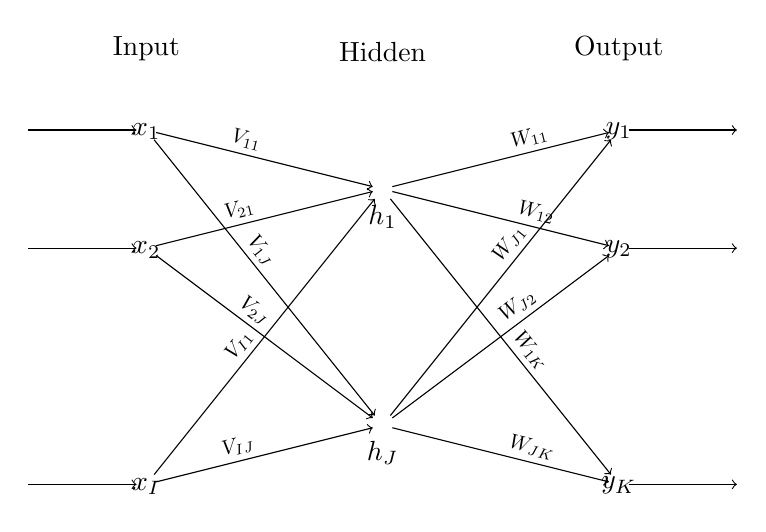
\begin{tikzpicture}[x=1.5cm,y=1.5cm]
	\foreach \m/\l [count=\y] in {1,2,missing,3}
		\node [every neuron/.try, neuron \m/.try] (input-\m) at (0,2-\y) {};
	\foreach \m [count=\y] in {1,missing,2}
		\node [every neuron/.try, neuron \m/.try] (hidden-\m) at (2,1.5-\y) {};
	\foreach \m/\l [count=\y] in {1,2,missing,3}
		\node [every neuron/.try, neuron \m/.try] (output-\m) at (4,2-\y) {};
	\foreach \l [count=\i] in {1,2,I}
		\draw [<-] (input-\i) -- ++(-1,0)
			node[above,xshift=1.5cm,yshift=-0.25cm] {$x_\l$};
	\foreach \l [count=\i] in {1,J}
		\node [above,yshift=-0.75cm] at (hidden-\i.north) {$h_\l$};
	\foreach \l [count=\i] in {1,2,K}
		\draw [->] (output-\i) -- ++(1,0)
			node[above,xshift=-1.5cm,yshift=-0.25cm] {$y_\l$};
	\foreach \a [count=\i] in {1,2,I}
		\foreach \b [count=\j] in {1,J}
			\draw [->] (input-\i) --
			(hidden-\j) node[midway,sloped,left,scale=0.75,yshift=0.25cm]
			{$V_{\a\b}$};
	\foreach \a [count=\i] in {1,J}
		\foreach \b [count=\j] in {1,2,K}
			\draw [->] (hidden-\i) --
			(output-\j) node[midway,sloped,left,scale=0.75,xshift=1cm,yshift=0.25cm]
			{$W_{\a\b}$};
	\node [align=center,above] at (0,1.5) {Input};
	\node [align=center,above] at (2,1.5) {Hidden};
	\node [align=center,above] at (4,1.5) {Output};
\end{tikzpicture}
\caption{\label{fig:caption} Netword layers}
\end{center}
\end{figure}

\subsection{Vocabulary architecture}

Vocabulary is stored in memory as BST. Each node has the following

\begin{itemize}
	\item word string
	\item vocabulary index
	\item number of occurences in a corpus file
	\item size of context BoW
	\item context BoW as linked list
	\item auxiliary pointers
\end{itemize}

\subsection{Parsing pipeline}

Parsing pipeline overview is as follows

\begin{algorithm}[H]
	\caption{Parsing pipeline}
	\SetAlgoStyle
	$vocab \gets$ BinarySearchTree()\;
	\For{$word$ \textbf{in} $vocab$}{
		clean($word$)\;
		\If{$word \notin stopWords$}{
			$center \gets$ createNode($word$)\;
			insertBST($vocab$, $center$)\;
			$window[C] \gets center$\;
			\For{$c \gets 0$ \textbf{to} $C-1$}{
				\If{$window[c] \neq center$}{
					insertList($center.context$, $window[c]$)\;
					insertList($window[c].context$, $center$)\;
				}
				$window[c] = window[c+1]$\;
			}
		}
	}
\end{algorithm}

Firstly, we are reading a corpus file, i.e. unfiltered file with raw
text. While we are doing that, we are cleaning the corpus by removing special
characters, numbers and stop words, and converting every word to it's
lowercase representation and, optionally, stemming it. As we said, unique words are stored in BST
vocabuary so we are going to perferm recursive, but preferably iterative,
insert operation. We are using window sliding technique to create context BoW 
for each center word by appending pointers to a linked list contained in the
corresponding BST node.

\medbreak

After reading the corpus file and populating BST with unique words, we need to
dynamically allocate required collection of structures in memory. Those
collections include

\begin{itemize}
	\item onehot word representation array
	\item input, hidden and output network layer
	\item input-hidden and hidden-output weight matrices
	\item prediction errors array
	\item training order array
	\item helper sampling matrix for NS phase
\end{itemize}

\medbreak

Then, we are populating hash map which is going to be used for asscociating
word and it's unique vocabulary index generated by preorder BST traversal.

\begin{algorithm}[H]
	\caption{Targets initialization}
	\SetAlgoStyle
	\Fn{target(node)}{
		\If{$node \neq NULL$}{
			$i \gets 0$\;
			\While{$node.context \neq NULL$}{
				$node.target[i] \gets tmp.word$\;
				$node.context \gets node.context.next$\;
				$i \gets i + 1$\;
			}
			delete($root.context$)\;
			target($noot.left$)\;
			target($node.right$)\;
		}
	}	
\end{algorithm}

\medbreak

After that, we need to calculated word frequency that will be needed
int the NS stage for random word sampling using Monte Carlo method inverse
proportional to it's frequency in order to lower the chances of sampling
high-frquency words.

\subsection{Weights initialization}

For now, we are using just a randomly sampled real numbers from uniform distrubution in the interval
$[0, 1]$. Prediction accuracy could potentially increase if we'd sample initial weight values from Gaussian
distrubution.

\subsection{Training pipeline}

Training phase consists of multiple epochs and in each one of them passing
every vocabulary word to input layer. We are not calculating loss function
because it's value is not required. Notice that we are done reading the file
and training phase is using only generated vocabulary from previous phase.
This results in training the network for a particular word only once and
independent of it's frequency.

\medbreak

To illustrate the idea mentioned above, let's compare original word2vec and our implementation.

\textbf{Original word2vec implementation.}
Initialize sliding window at the beginning of the file. For each center word $\boldsymbol{x}$, create context BoW $\boldsymbol{C}$. For each context word $\boldsymbol{c_i} \in \boldsymbol{C}$, run training for pair $(\boldsymbol{x}, \boldsymbol{c_i})$ and calculate error vector $\boldsymbol{e}$ at the output layer. This way we run $|\boldsymbol{C}|$ training passes for each center word.

\textbf{Our implementation.}
Given a vocabulary $\mathcal{V}$, for each $\boldsymbol{x} \in \mathcal{V}$ run training for pair $(\boldsymbol{x}, \boldsymbol{C})$, where $\boldsymbol{C}$ is a context BoW of center word $\boldsymbol{x}$. This way we run only one training pass for each center word.

Training pipeline overview is as follows

\begin{algorithm}[H]
	\caption{Training pipeline}
	\SetAlgoStyle
	\For{$epoch \gets 0$ \textbf{to} $EPOCH\_MAX$}{
		$vocab \gets$ shuffle(vocab)\;
		\For{$word$ \textbf{in} $vocab$}{
			propagateForward()\;
			sampleNegatives()\;
			normalizeOutput()\;
			calculateError()\;
			propagateBackward()\;
		}
		sarializeWeights()\;
	}
\end{algorithm}

\subsection{Testing pipeline}

Testing pipeline overview is as follows

\begin{algorithm}[H]
	\caption{Testing pipeline}
	\SetAlgoStyle
	$success \gets 0$\;
	$total \gets 0$\;
	\For{$word$ \textbf{in} $test$}{
		clean($word$)\;
		\If{$word \notin stopWords$}{
			propagateForward()\;
			normalizeOutput()\;
			$pred \gets argmax(output)$\;
			\If{$word = pred$}{
				$success \gets success + 1$\;
			}
			$total \gets total + 1$\;
		}
	}
	$acc \gets success / total$\;
\end{algorithm}

\subsection{Process of learning}

Forawrd propagation of input is done as follows

\begin{align}
	&h_j = \sum_{i=1}^I (x_i \cdot V_{ij}) \\
	&y_k = \sum_{j=1}^J (h_j \cdot W_{jk}) \\
	&t_k =
	\begin{cases}
		1, &\text{if } \boldsymbol{\mathcal{V}_k} \in \boldsymbol{C} \\
		0, &\text{otherwise}
	\end{cases} \\
	&e_k = y_k - t_k \\
	&l_j = \sum_{k=1}^K (e_k \cdot W_{jk}) \\
	&\begin{aligned}
		E &= -\log P(x_{c_1}, x_{c_2},\ldots,x_{c_C}|x_0) \\
		&= -\log \prod_{c=1}^C P(x_{c_i}|x_0) \\
		&= -\log \prod_{c=1}^C softmax(\boldsymbol{y_c}) \\
		&= -\log \prod_{c=1}^C \frac{e^{y_{c_{k^\prime}}}}{\sum_{k=1}^K
		e^{y_{c_k}}} \\
		&= \sum_{c=1}^C \log\sum_{k=1}^K e^{y_{c_k}} - \sum_{c=1}^C
		y_{c_{k^\prime}}
	\end{aligned}
\end{align}

where $k^\prime$ is and index of $c^{th}$ context word

\begin{algorithm}[H]
	\caption{Forward propagation of input}
	\SetAlgoStyle
	\Fn{propagateForward()}{
		\For{$j \gets 0$ \textbf{to} $J$}{
			$h[j] \gets 0$\;
			\For{$i \gets 0$ \textbf{to} $I$}{
				$h[j] \gets h[j] + x[i] \cdot V[i, j]$\;
			}
		}
		\For{$k \gets 0$ \textbf{to} $K$}{
			$y[j] \gets 0$\;
			\For{$j \gets 0$ \textbf{to} $J$}{
				$y[j] \gets y[j] + h[i] \cdot W[j, k]$\;
			}
		}
	}
\end{algorithm}

Error calculation is as follows

\begin{algorithm}[H]
	\caption{Error calculation}
	\SetAlgoStyle
	\Fn{calculateError()}{
		\For{$k \gets 0$ \textbf{to} $K$}{
			$e[k] \gets 0$\;
			\For{$c$ \textbf{in} $context$}{
				$e[k] \gets e[k] + output[k]$\;
				\If{$k = indexOf(c)$}{
					$e[k] \gets e[k] - 1$\;
				}
			}
		}
	}
\end{algorithm}

Backward error propagation is done using relationships defined by

\begin{align}
	&W_{jk}^\prime = W_{jk} - \alpha \cdot \frac{\partial E}{\partial W_{jk}} =
	W_{jk} - \alpha \cdot e_k \cdot h_j \\
	&V_{ij}^\prime = V_{ij} - \alpha \cdot \frac{\partial E}{\partial V_{ij}} =
	V_{ij} - \alpha \cdot l_j
\end{align}

where $\alpha$ is a learning rate hyperparameter which is decreasing as
training progresses using simulated annealing technique.

\begin{algorithm}[H]
	\caption{Backward propagation of error}
	\SetAlgoStyle
	\Fn{propagateBackward()}{
		\For{$j \gets 0$ \textbf{to} $J$}{
			$eh \gets 0$\;
			\For{$k \gets 0$ \textbf{to} $K$}{
				$W[j, k] \gets W[j, k] - \alpha \cdot e[k] \cdot h[j]$\;
				$eh \gets eh + e[k] \cdot W[j, k]$\;
			}
			$V[i, j] \gets V[i, j] - \alpha \cdot eh$\;
		}
	}
\end{algorithm}

Partial derrivatives we've used are as follows

\begin{align}	
	&\frac{\partial E}{\partial W_{jk}} = \sum_{c=1}^C \sum_{k=1}^K
	\frac{\partial E}{\partial y_{c_k}} \cdot \frac{\partial y_{c_k}}{\partial
	W_{jk}} \\
	&\frac{\partial E}{\partial V_{ij}} = \sum_{c=1}^C \sum_{k=1}^K
	\frac{\partial E}{\partial y_{c_k}} \cdot \frac{\partial y_{c_k}}{\partial
	V_{ij}}
\end{align}

\subsection{Hyperparameters}

We are using hyperparameters defined below to tweak our network in order to get the best accuracy and performance.

\begin{itemize}
	\item $J$ - Number of neurons in the hidden layer
	\item $EPOCH\_MAX$ - Total epochs per training
	\item $C$ - Size of sliding window, i.e. size of context BoW
	\item $WEIGHT\_MAX$ - Upper bound for initial weight value sampling
	\item $ALPHA\_MAX$ - Initial learning rate value
	\item $ALPHA\_MIN$ - Final learning rate value
	\item $SAMPLES\_MAX$ - Number of negative samples to pick
	\item $SAMPLE\_FACTOR$ - Average normalized frequency of every word
	\item $SAMPLE\_EXIT$ - Upper bound for unsuccessful samplings
\end{itemize}

\medbreak

Value for $J$ hyperparameter would preferably be selected using an algorithm proposed by Branislav Milojković.

\subsection{Negative sampling}

Implementation in progress.

\section{Vector representations of sentences}

Word embeddings on their own are useful for analyzing relationships between
words, but encoding sentences can give us better semantic understanding of
larger chunks of text. Sentence encoding is done as follows

\begin{algorithm}[H]
	\caption{Sentence encoding}
	\SetAlgoStyle
	\Fn{encode(sentence)}{
		\For{$word$ \textbf{in} $sentence$}{
			clean($word$)\;
			\If{$word \notin stopWords$}{
				$i \gets$ indexOf($word$)\;
				\For{$j \gets 0$ \textbf{to} $J$}{
					$vec[j] \gets vec[j] + V[i][j]$\;
				}
			}
		}
		\Return{$vec$}\;
	}
\end{algorithm}

\section{Fast tests}

What if we don't use a $softmax$ function or, better yet, a whole network? What if
we can predict next word just by running statistical test on our vocabulary?

\begin{align}	
	&\begin{aligned}	
		E &= -\log P(x_{c_1}, x_{c_2},\ldots,x_{c_C}|x_0) \\
		&= -\log \prod_{c=1}^C P(x_{c_i}|x_0) \\
		&= -\log \prod_{c=1}^C \frac{P(x_{c_i}x_0)}{P(x_0)} \\
		&= -\log \prod_{c=1}^C \frac{\phi_{x_0}(x_{c_i})}{\phi(x_0)}
	\end{aligned}
\end{align}

where $\phi(x_i)$ denotes normalized or even better
non-normalized (arithmetic underflow problem) frequency of
a word $x_i$ and $\phi_{x_0}(x_{c_i})$ denotes frequency of
a word $x_{c_i}$ in context BoW of a word $x_0$

What if we use some rules to score each word in a context BoW? Can we agree
on the following hypothesis?

\medbreak

\textit{Context word just before a given center word has a
higher impact on classification result than a word which is $n$ places after our
center word.}

\section{Results and discussion}

\fig{chart}{Very useful dot}

\end{document}
